% Clean grid redraw of plots/mismatch/2_1/explaining_network_2_1.gml
% (the BIC-cherry "explaining network" for hybrid_network_2_1.gml, task_1d.py step 3).
%
% Structural fact this layout exploits: the 16 "p_X_Y" nodes are exactly the
% complete pairing of the 4 blue leaves with the 4 orange leaves (a K_{4,4}).
% Placing them in a 4x4 grid (columns = blue leaves, rows = orange leaves)
% makes every parent->leaf edge purely horizontal or vertical, and -- as a
% bonus -- every parent->parent ("nested cherry") edge turns out to run
% exactly along one row or one column too. Each grid column/row is therefore
% drawn as a single "metro line" (solid black, one arrowhead at the leaf
% header) that all nodes on that line implicitly feed into.
%
% Compile with: pdflatex explaining_network_2_1_clean.tex
\documentclass{article}
\usepackage[margin=1cm]{geometry}
\usepackage{tikz}
\usetikzlibrary{arrows.meta}

% matplotlib tab:blue / tab:orange, matching the gene_color values in the GML
\definecolor{tabblue}{rgb}{0.12156863,0.46666667,0.70588235}
\definecolor{taborange}{rgb}{1.0,0.49803922,0.05490196}

\begin{document}
\thispagestyle{empty}
\begin{center}
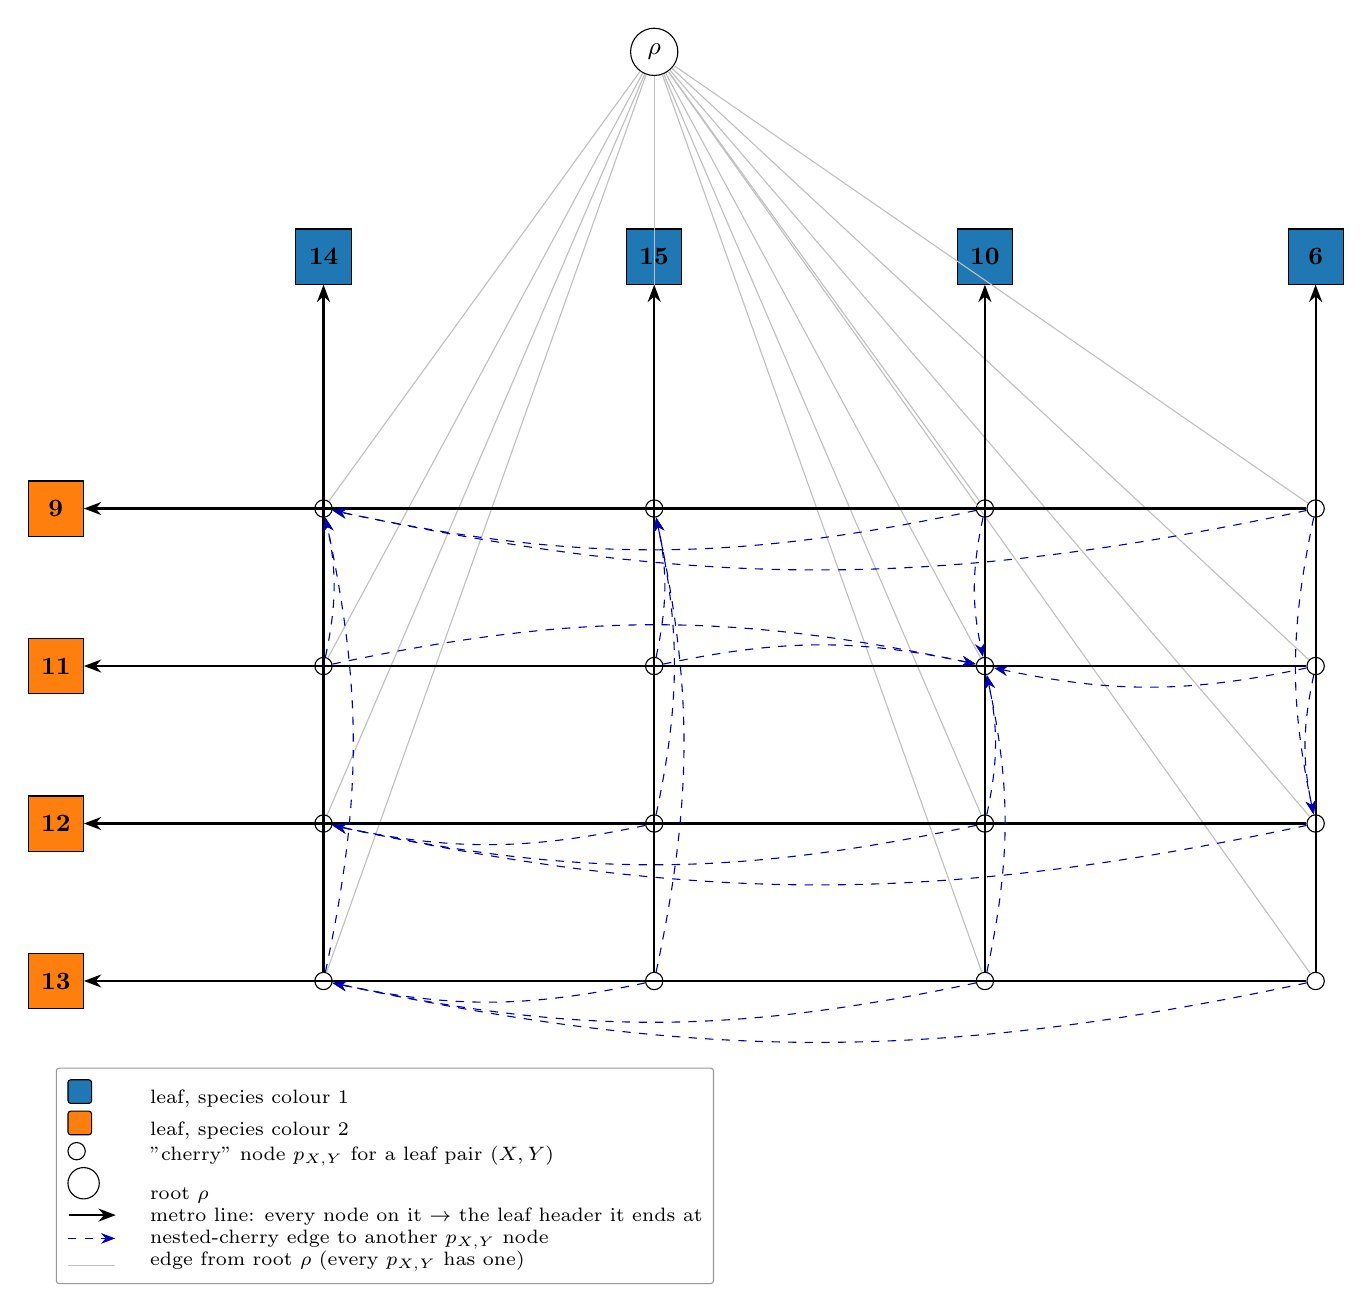
\begin{tikzpicture}[
  >={Stealth[length=2.2mm]},
  every node/.style={font=\small\bfseries},
  leafblue/.style={rectangle, fill=tabblue, text=black, minimum size=7mm, draw=black},
  leaforange/.style={rectangle, fill=taborange, text=black, minimum size=7mm, draw=black},
  rootnode/.style={circle, draw=black, fill=white, minimum size=6mm, font=\small},
  parentnode/.style={circle, draw=black, fill=white, minimum size=2.2mm, inner sep=0pt},
  rail/.style={-{Stealth[length=2.2mm]}, thick},
  rootedge/.style={-, thin, black!25},
  nestedge/.style={-{Stealth[length=1.8mm]}, thin, blue!70!black, dashed},
]

% ---- blue leaf headers (top) ----
\node[leafblue] (b14) at (0, 0) {14};
\node[leafblue] (b15) at (4.2, 0) {15};
\node[leafblue] (b10) at (8.4, 0) {10};
\node[leafblue] (b6) at (12.6, 0) {6};
% ---- orange leaf headers (left) ----
\node[leaforange] (o9) at (-3.4, -3.2) {9};
\node[leaforange] (o11) at (-3.4, -5.2) {11};
\node[leaforange] (o12) at (-3.4, -7.2) {12};
\node[leaforange] (o13) at (-3.4, -9.2) {13};
% ---- root ----
\node[rootnode] (rho) at (4.2, 2.6) {$\rho$};
% ---- 16 parent grid nodes (rows = orange leaf, cols = blue leaf) ----
\node[parentnode] (p9)  at (0,-3.2)  {};
\node[parentnode] (p10) at (0,-5.2)  {};
\node[parentnode] (p11) at (0,-7.2)  {};
\node[parentnode] (p12) at (0,-9.2)  {};
\node[parentnode] (p13) at (4.2,-3.2) {};
\node[parentnode] (p14) at (4.2,-5.2) {};
\node[parentnode] (p15) at (4.2,-7.2) {};
\node[parentnode] (p16) at (4.2,-9.2) {};
\node[parentnode] (p17) at (8.4,-3.2) {};
\node[parentnode] (p18) at (12.6,-3.2){};
\node[parentnode] (p19) at (8.4,-5.2) {};
\node[parentnode] (p20) at (8.4,-7.2) {};
\node[parentnode] (p21) at (8.4,-9.2) {};
\node[parentnode] (p22) at (12.6,-5.2){};
\node[parentnode] (p23) at (12.6,-7.2){};
\node[parentnode] (p24) at (12.6,-9.2){};

% ---- root -> every parent (thin, de-emphasised; drawn first, underneath) ----
\draw[rootedge] (rho) -- (p9);
\draw[rootedge] (rho) -- (p10);
\draw[rootedge] (rho) -- (p11);
\draw[rootedge] (rho) -- (p12);
\draw[rootedge] (rho) -- (p13);
\draw[rootedge] (rho) -- (p14);
\draw[rootedge] (rho) -- (p15);
\draw[rootedge] (rho) -- (p16);
\draw[rootedge] (rho) -- (p17);
\draw[rootedge] (rho) -- (p18);
\draw[rootedge] (rho) -- (p19);
\draw[rootedge] (rho) -- (p20);
\draw[rootedge] (rho) -- (p21);
\draw[rootedge] (rho) -- (p22);
\draw[rootedge] (rho) -- (p23);
\draw[rootedge] (rho) -- (p24);

% ---- "metro lines": every node on a column line feeds its blue header; ----
% ---- every node on a row line feeds its orange header (32 edges, 8 lines) ----
\draw[rail] (p12) -- (b14);
\draw[rail] (p16) -- (b15);
\draw[rail] (p21) -- (b10);
\draw[rail] (p24) -- (b6);
\draw[rail] (p18) -- (o9);
\draw[rail] (p22) -- (o11);
\draw[rail] (p23) -- (o12);
\draw[rail] (p24) -- (o13);

% ---- nested-cherry (parent -> parent) edges: bowed out so they read apart ----
% ---- from the straight metro lines they run alongside ----
\draw[nestedge] (p10) to[bend right=12] (p9);
\draw[nestedge] (p10) to[bend left=12] (p19);
\draw[nestedge] (p12) to[bend right=12] (p9);
\draw[nestedge] (p14) to[bend right=12] (p13);
\draw[nestedge] (p14) to[bend left=12] (p19);
\draw[nestedge] (p15) to[bend right=12] (p13);
\draw[nestedge] (p15) to[bend left=12] (p11);
\draw[nestedge] (p16) to[bend right=12] (p13);
\draw[nestedge] (p16) to[bend left=12] (p12);
\draw[nestedge] (p17) to[bend left=12] (p9);
\draw[nestedge] (p17) to[bend right=12] (p19);
\draw[nestedge] (p18) to[bend left=12] (p9);
\draw[nestedge] (p18) to[bend right=12] (p23);
\draw[nestedge] (p20) to[bend right=12] (p19);
\draw[nestedge] (p20) to[bend left=12] (p11);
\draw[nestedge] (p21) to[bend right=12] (p19);
\draw[nestedge] (p21) to[bend left=12] (p12);
\draw[nestedge] (p22) to[bend left=12] (p19);
\draw[nestedge] (p22) to[bend right=12] (p23);
\draw[nestedge] (p23) to[bend left=12] (p11);
\draw[nestedge] (p24) to[bend left=12] (p12);

% ---- legend ----
\node[anchor=north west, font=\scriptsize, align=left, draw=black!40, fill=white, inner sep=4pt, rounded corners=1pt]
  at (-3.4, -10.3) {%
  \begin{tabular}{@{}ll@{}}
    \tikz\node[leafblue, minimum size=3mm]{};   & leaf, species colour 1 \\
    \tikz\node[leaforange, minimum size=3mm]{}; & leaf, species colour 2 \\
    \tikz\node[parentnode]{};                    & "cherry" node $p_{X,Y}$ for a leaf pair $(X,Y)$ \\
    \tikz\node[rootnode, minimum size=3mm, font=\tiny]{};& root $\rho$ \\
    \tikz\draw[rail] (0,0) -- (0.6,0);           & metro line: every node on it $\to$ the leaf header it ends at \\
    \tikz\draw[nestedge] (0,0) -- (0.6,0);        & nested-cherry edge to another $p_{X,Y}$ node \\
    \tikz\draw[rootedge] (0,0) -- (0.6,0);        & edge from root $\rho$ (every $p_{X,Y}$ has one) \\
  \end{tabular}%
};

\end{tikzpicture}
\end{center}
\end{document}
